% Integration snippets for ThesisProj-2.pdf (nine-page manuscript).
% These do not replace the repository's different, longer manuscript.
% Requires amsmath, amssymb, graphicx and booktabs already used by the paper.
% Copy plot PDFs into the same directory as the manuscript or adjust paths.

% ABSTRACT: replace the existing abstract with a scoped empirical claim.
\begin{abstract}
We investigate when spatial structure improves magnitude-only channel
estimation for Rydberg atomic receivers with a known reference field.
A Hankel-structured extension of expectation--maximization Gerchberg--Saxton
(EM-GS) selects a shared structural order from held-out pilots and refits
the channel using all pilots. Independent simulations give an average
paired-median improvement of 2.70~dB over EM-GS at the principal operating
point. The benefit increases with array capacity and decreases with
multipath complexity; at high complexity, forced rank reduction can be
harmful. Normalized effective rank organizes these trends, but does not
define a universal performance threshold, and normalized path count is a
stronger predictor on the tested matched geometric-channel configurations.
Positive gains also persist under two alternative multipath distributions.
A controlled comparison with matching Cadzow sweeps finds a modest
advantage for interleaving the structural step, while rank selection remains
the dominant computational cost for larger arrays.
\end{abstract}

% SYSTEM MODEL: the current PDF's equation (9) has no left-hand side.
\begin{equation}
\mathbf E=\mathbf G\mathbf S+\mathbf B+\mathbf W,
\qquad \mathbf Z=|\mathbf E|.
\end{equation}

% Replace the final SNR/RSR paragraph of Section II.
We define SNR using the aggregate received signal power from all users:
\begin{equation}
\mathrm{SNR}=\frac{c^2\sum_{k=1}^{K}\beta_k}{\sigma^2}.
\end{equation}
The reference-to-signal ratio uses a single-user reference power. In the
equal-power simulations, $c=1$ and $\beta_k=1$, so
$\sigma^2=K/10^{\mathrm{SNR}_{\mathrm{dB}}/10}$ and the reference magnitude
is $10^{\mathrm{RSR}_{\mathrm{dB}}/20}$. All SNR axes use this aggregate
convention.

% ESTIMATOR: insert actual update equations instead of relying only on the
% singular-value example. Keep the explanation concise around these equations.
Starting from the spectral initialization, the EM update is
\begin{align}
\boldsymbol\Lambda^{(t)}&=\mathbf G^{(t)}\mathbf S+\mathbf B,\\
\mathbf K^{(t)}&=2\mathbf Z\odot|\boldsymbol\Lambda^{(t)}|/\sigma^2,\\
\mathbf Y^{(t)}&=\mathbf Z\odot R(\mathbf K^{(t)})
 \odot\exp\!\left(\mathrm{j}\arg\boldsymbol\Lambda^{(t)}\right),\\
\widetilde{\mathbf G}^{(t+1)}&=(\mathbf Y^{(t)}-\mathbf B)
 \mathbf S^H(\mathbf S\mathbf S^H)^{-1},
\end{align}
where $R(x)=I_1(x)/I_0(x)$ is applied elementwise and $\odot$ denotes
elementwise multiplication. For each user column, HS-GS then applies four
Cadzow sweeps to $\widetilde{\mathbf G}^{(t+1)}$. Each sweep truncates the
Hankel matrix to the selected rank and averages its antidiagonals. These
finite sweeps exploit a low-rank structural surrogate; they are not an
exact projection onto all physical constraints of the geometric channel.

% Replace the rank-selection subsection with this operational description.
\subsection{Choosing the Hankel Rank}
The true path count is not used for rank selection. We reserve the final
$\max(1,\operatorname{round}(0.3P))$ pilot columns for validation and fit
each candidate rank $r\in\{1,\ldots,r_{\max}\}$ using the remaining columns.
The candidate minimizing the sum of squared magnitude residuals on the
validation columns is selected. One scalar rank is shared across the user
columns. After selection, the final estimator is initialized again and
fitted using \emph{all} $P$ pilots. Candidate and final iteration budgets
are listed separately for each experiment. If the selected rank is
$r_{\max}$, the structural step is bypassed and the final estimate equals
the paired EM-GS estimate. This fallback is exact, but rank selection does
not guarantee that an active constraint improves every individual trial.

% EXPERIMENTAL SETUP: use in place of the opening numerical-results paragraphs.
The independent verification comprises 27,300 paired Monte Carlo trials
across 73 operating cells, with 300 or 400 trials per cell. Within each
trial, all estimators use the same channel, pilots, reference and noise.
The principal comparison uses $N=32$, $K=3$, $P=30$, RSR $=12$~dB,
100 final iterations and 25 iterations per candidate rank, with four
Cadzow sweeps per application. The path-count sweep uses 50 final and
20 candidate iterations. Matched effective-rank experiments use $P=20$,
RSR $=10$~dB, 100/25 iterations and SNR drawn uniformly from $[-10,20]$~dB
on a millidecibel grid. Trial counts are fixed before simulation.

We distinguish the ratio-of-sums NMSE used for error curves from the median
paired improvement. Writing $e_{m,i}=\|\widehat{\mathbf G}_{m,i}
-\mathbf G_i\|_F^2$ and $d_i=\|\mathbf G_i\|_F^2$, these are
\begin{align}
\mathrm{NMSE}_{m,\mathrm{dB}}&=10\log_{10}
 \frac{\sum_i e_{m,i}}{\sum_i d_i},\\
\Delta_{\mathrm{med}}&=\operatorname{median}_i
 \left[10\log_{10}\frac{e_{\mathrm{EM},i}}{e_{\mathrm{HS},i}}\right].
\end{align}
Pointwise 95\% confidence intervals use 4,000 paired bootstrap resamples.
Pooled random-SNR medians are conditional on the stated SNR distribution.

% PERFORMANCE AGAINST BOUNDS: replace exact numerical claims together.
At the principal operating point, the per-SNR paired-median gains range
from 2.54 to 2.97~dB, with a six-point mean of 2.70~dB. The corresponding
vertical gaps between the ratio-of-sums NMSE curves range from 2.38 to
2.90~dB. Projection is active in all 2,400 principal trials. The Rician
CRLB and geometric CCRB are evaluated on these same channel realizations
and normalized by the same channel-energy sums. At SNRs of 5~dB and
above, EM-GS differs from the Rician CRLB by at most 0.107~dB. The CCRB
is 6.95--7.06~dB below the unconstrained bound, and HS-GS remains
4.37--4.85~dB above the CCRB. These are unbiased-estimator reference
curves, not unconditional lower limits for the biased estimators tested.

% ARRAY TABLE: replace the existing numerical table.
\begin{center}
\begin{tabular}{rrrr}
\toprule
$N$ & Ratio-of-sums gain & Paired-median gain & EM-GS NMSE\\
\midrule
8 & $-0.095$ & $0.236$ & $-8.666$\\
16 & $0.866$ & $1.044$ & $-8.786$\\
32 & $2.938$ & $3.264$ & $-8.733$\\
\bottomrule
\end{tabular}
\end{center}
All entries are in decibels and average the twelve operating-point
summaries. At $N=8$, projection is inactive in 42.94\% of trials.
The averaged EM-GS baseline spans only 0.120~dB across these array sizes.

% PATH COMPLEXITY: replace the endpoint/numerical conclusions.
At fixed $N=32$ and SNR $=5$~dB, the ratio-of-sums gain decreases from
7.377~dB, with a 95\% interval of $[7.162,7.607]$~dB, at $L=2$ to
$-0.125$~dB, with interval $[-0.204,-0.046]$~dB, at $L=16$.
The paired median at $L=16$ is zero, illustrating that typical-trial
improvement and aggregate squared error need not give the same summary.
The EM-GS baseline spans only 0.129~dB in this experiment.

% EFFECTIVE RANK: replace the crossing and universal-cutoff paragraphs.
Normalized effective rank is computed from the true noiseless channel and
is used only for retrospective analysis. Repeating the original Figure~3
construction yields crossing estimates of 0.580, 0.509 and 0.526 for
$N=16,32,64$. The $N=16$ and $N=64$ values are extrapolations from three
positive-gain points, whereas the $N=32$ value interpolates between
positive and negative point estimates. They should not be interpreted as
three directly observed thresholds. Additional high-complexity cases
approach a zero-median plateau, partly due to exact EM-GS fallback.

For the main effective-rank comparison, we therefore match the pilot count,
RSR, iteration budgets, SNR distribution and pooled-median statistic across
all three array sizes. In these matched experiments, $N=32$ retains a
median gain of 0.141~dB at $\rho=0.536$, with interval $[0.090,0.211]$~dB.
The results support a declining benefit with increasing complexity, but
do not establish a universal cutoff at $\rho=0.5$.

Using the matched $N=32$ curve to predict six held-out $N=16$ and $N=64$
configurations, the mean absolute errors are 2.067~dB for raw path count,
0.073~dB for normalized path count $L/r_{\max}$, and 0.317~dB for
normalized effective rank. Thus effective rank improves on raw path count
in this test but is not the strongest of the tested descriptors. This
comparison is conditional on the tested configurations and interpolation
scheme; all six target gains are positive.

At $N=16$, $L=14$ and measured $\rho=0.732$, forcing rank seven produces
a median gain of $-0.154$~dB with interval $[-0.201,-0.111]$~dB.
Adaptive HS-GS has zero pooled median gain in the same trials. This
demonstrates a risk of forced rank reduction without implying that
adaptive selection is harmless in every realization.

% TRANSFER: preserve frozen predictions; do not refit them on the new results.
The two additional distributions yield positive median gains in 400 fresh
trials each. The clustered channel has measured $\rho=0.335$ and gain
1.182~dB with interval $[0.995,1.398]$~dB. Its error relative to the
previously frozen 1.300~dB prediction is 0.118~dB. The ten-path channel
has measured $\rho=0.407$ and gain 0.831~dB with interval
$[0.710,1.011]$~dB; its error relative to the frozen 0.648~dB prediction
is 0.183~dB. These results support positive structural gains across the
two tested distributions, but not exact predictive calibration. Both
distributions remain within the geometric ULA model. Initial gains have
variance $1/D$ for $D$ rays, followed by whole-channel scaling to match
the realized total power of a base channel draw. The clustered model uses
four clusters with ten rays per cluster, uniform $\pm5^\circ$ offsets,
and clipping to the allowed angle interval.

% USER COUNT / RUNTIME: disclose the jointly changing quantities.
At SNRs of 5~dB and above, median gains are 3.381, 3.509 and 3.552~dB for
$K=2,3,4$. These cases use $P=13,20,27$, respectively, and $L=5$,
maintaining approximately constant $P/(2K)$ under aggregate SNR. The
0.170~dB span therefore describes this joint design rather than varying
$K$ alone. Serial timing of the production implementation gives median
rank-selection shares of 47.5\%, 65.3\%, 79.3\% and 88.5\% for
$N=8,16,32,64$ at $P=20$ and SNR $=5$~dB. These measurements use three
trials per point and depend on hardware and implementation. Report the
platform and software versions alongside the timing table.

% PLACEMENT: replace the final numerical-results paragraph.
The original comparison, using four sweeps per interleaved application
and one final sweep, gives a mean of six per-SNR median differences of
$-0.012$~dB, with a stratified-bootstrap interval of $[-0.049,0.034]$~dB.
It changes both placement and sweep count. With four sweeps per application
in both variants, interleaving gains 0.204~dB on average, with interval
$[0.169,0.242]$~dB; with one sweep in both variants, the corresponding
gain is 0.239~dB, with interval $[0.204,0.282]$~dB. All variants share
the rank selected using four-sweep interleaved candidates, so these are
conditional comparisons rather than separately tuned estimators.
Matching sweeps per application also does not match total computation.
The two placements produce different estimates: the median distance
between interleaved-four and final-one estimates is 0.532 times the true
channel norm at $-5$~dB and 0.022 at 20~dB. The controlled results support
a modest placement effect rather than identical outputs or established
equivalence.

% FIGURE INTEGRATION EXAMPLES (place within the relevant figure environments).
% 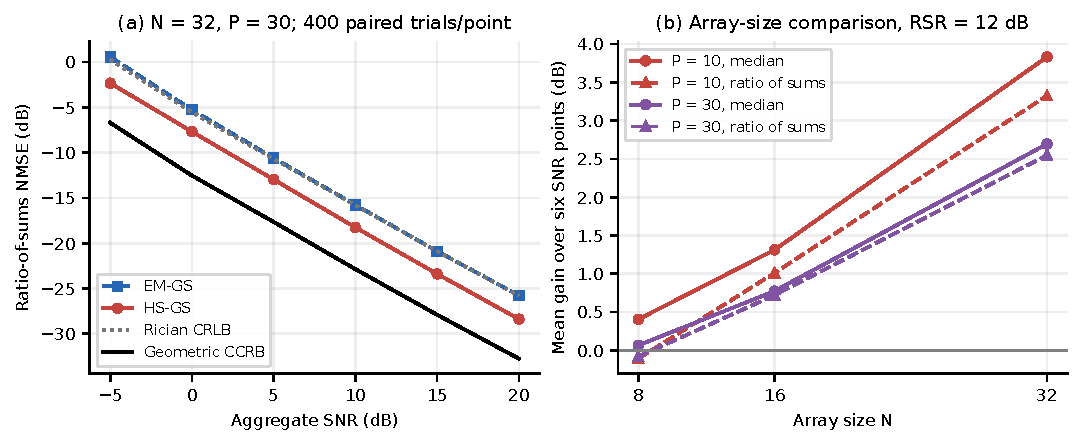
\includegraphics[width=\textwidth]{figure2_performance_array.pdf}
% 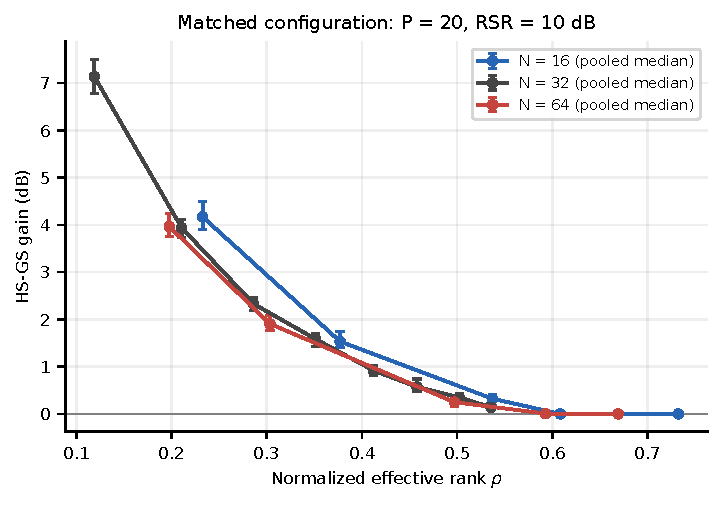
\includegraphics[width=\columnwidth]{figure3_matched.pdf}
% 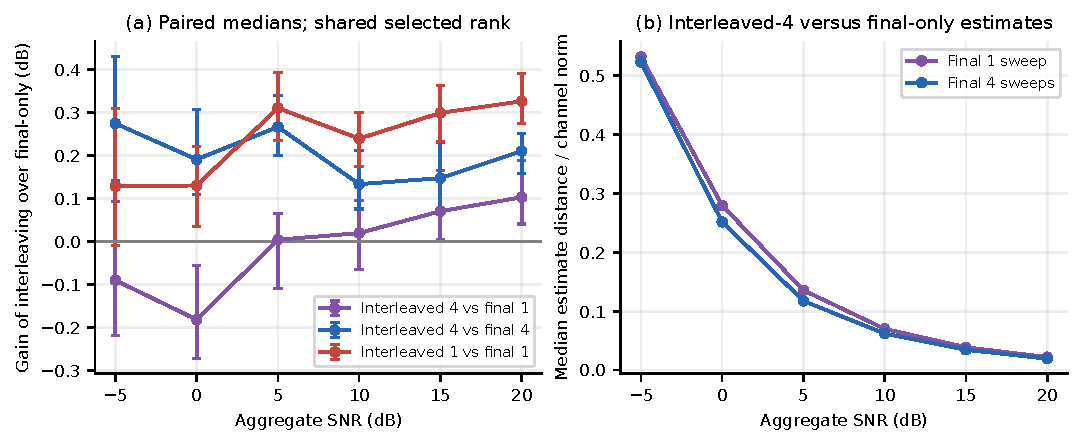
\includegraphics[width=\textwidth]{projection_placement.pdf}

% CONCLUSION: retain these limits when editing the rest of the conclusion.
The independent simulations support exploiting Hankel structure when the
channel is simple relative to array capacity. The gain declines as channel
complexity increases, and forced rank reduction can be harmful. Normalized
effective rank is a useful descriptive coordinate, but normalized path
count is a stronger predictor on the tested matched geometric channels,
and no universal threshold has been established. Matching-sweep experiments
show a modest advantage for interleaving the structural step, at additional
computational cost. These conclusions apply to the specified simulated
ULA magnitude-observation model; they have not been validated using
measured Rydberg hardware data.
